\graphicspath{ {Figures/chapter01} }
\section{Background and overview}
Control theory is a multidisciplinary field that plays a pivotal role in engineering and technology, providing a systematic framework for understanding, analyzing, and designing systems to achieve desired behaviors. At its core, control theory aims to regulate the output of a system, ensuring it conforms to a specified reference or trajectory. This field has far-reaching applications, ranging from industrial processes and aerospace systems to biological and economic systems.

The origins of control theory can be traced back to the early 19th century, with the advent of steam engines and the industrial revolution. Engineers faced challenges in maintaining the stability and efficiency of these complex mechanical systems. James Clerk Maxwell, a Scottish physicist, made early contributions with his Paper On governor—a mechanical device designed to regulate the speed of steam engines \cite{maxwell1868governors}. This marked the beginning of a systematic approach to controlling systems.

In the early 20th century, Norbert Wiener, a mathematician, and engineer, introduced the concept of cybernetics—a term derived from the Greek word for "steersman." Wiener's work focused on feedback systems and communication in both biological and mechanical systems. His seminal work, "Cybernetics: Or Control and Communication in the Animal and the Machine" (1948) \cite{wiener2019cybernetics}, provided a theoretical foundation for control theory.

Simultaneously, Aleksandr Lyapunov, a Russian mathematician, developed the theory of stability, which became a cornerstone in the analysis of dynamic systems. Lyapunov's stability theory laid the groundwork for understanding when a system would remain stable over time, a critical aspect of control system design \cite{lyapunov1992general}. 

The mid-20th century witnessed a surge in the formalization of control theory. Engineers and mathematicians began developing mathematical models and techniques to analyze and design control systems. Notable contributors during this period include Rudolf Kalman, who introduced the Kalman filter for state estimation \cite{kalman1960contributions}, and Richard Bellman, who pioneered dynamic programming as a method for solving optimization problems in control systems \cite{bellman1966dynamic}. The advent of computers in the 1950s and 1960s revolutionized control theory by enabling the implementation of complex algorithms for real-time control. This era also saw the rise of the field of optimal control.

In the latter half of the 20th century, control theory continued to evolve with the introduction of robust control techniques, adaptive control strategies, and the application of control theory to non-linear systems. The field expanded its reach into aerospace engineering, telecommunications, and other emerging technologies.

Today, control theory remains a dynamic and evolving field, with the ongoing researches into advanced control methodologies, researchers are in dire need of a real system on which to test advanced control methods and thesis.
The implementation of control systems in unstable physical systems is a critical aspect of engineering, as it addresses the need to stabilize systems that are prone to catastrophic failures. Textbooks on control systems often feature example problems involving such unstable systems, providing students with opportunities to study their behavior and explore various methods for designing and implementing control algorithms.

Two well-known examples of unstable systems used experimentally are the inverted pendulum and ball balancing systems on beams that shown in figure 1.1 or ball and plate. These systems serve as valuable educational tools, allowing students to understand the challenges associated with instability and the importance of control in maintaining stability. The study of these systems provides a foundation for exploring different control strategies and algorithms.

The ball and plate system (BPS) represents a extended and generalized version of the traditional ball and beam. In this system, a ball can freely roll on a rigid platform, and the inclination of the platform can be independently manipulated in two directions. 
\begin{figure}
    \centering
    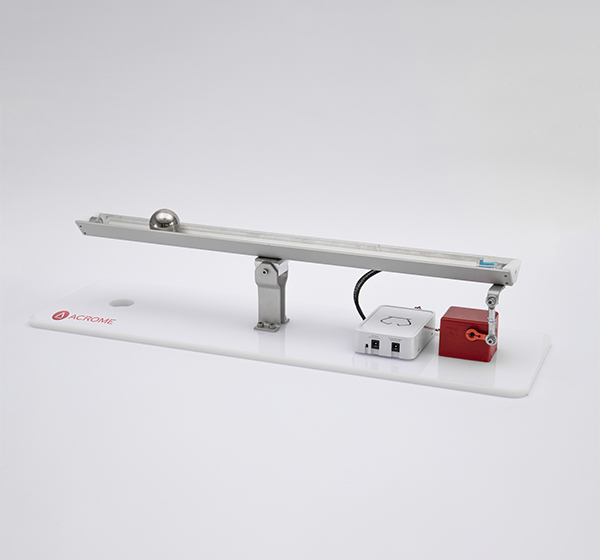
\includegraphics[width=0.7\linewidth]{ball-and-beam-new.jpg}
    \caption{Ball and Beam system}
    \label{fig:enter-label}
\end{figure}
The rigid plate, often equipped with a resistive touch panel or a camera, measures the position of the ball with respect to the center or a predetermined point on the plate. This system, by its nature, is inherently unstable, as even a minor disturbance can cause the ball to deviate significantly from its stationary position. Moreover, it lacks the ability to naturally return to equilibrium without external force intervention, which necessitating control methods for stability.

Everything we mentioned previously, in addition to the fact that the system is easily transportable, affordable, safe, has few malfunctions, scalable and controllable makes the BPS an ideal practical test environment for evaluating control methods in real-world scenarios. The main goal of the system is to keep the ball balanced on the plate within set boundaries or specific points. When the ball goes beyond these limits, a controller steps in, adjusting the plate's tilt in two directions to bring the ball back to its intended position.

To work effectively with the BPS, creating a precise nonlinear model is crucial for implementing model-based controllers. The Lagrange-Euler method is commonly used to derive the system's nonlinear equations by considering the kinetic and potential energies. Kinetic energy accounts for both linear and angular motions, while potential energies are calculated for all rigid bodies in the system. This method ensures a thorough understanding of the system's dynamics, facilitating the design and optimization of controllers tailored to its specific behavior.
 In our thesis we will work to design three different controllers to control the system theoretically and we will implement a PID controller to control the system experimentally then we will make a performance response comparison between these controllers.
 
\section{Literature review}
In general the previous works on ball-on-plate system can be classified based on several categories, Based on the type of the sensor used, based on actuation and linkage prototype or based on the controllers used to stabalize the system.

In \cite{awtar2002mechatronic}, \cite{ham2015development} Awtar and Ham introduced a prototype with a resistive touch screen and servo-motors for plate deflection. Another method in\cite{madhumitha2021design}, \cite{zhao2014multiple}, \cite{han2012tracking} and \cite{bdoor2016design} used a top-positioned camera for ball location extraction, while Debono \cite{debono2015application} employed a camera and computer algorithm for faster acquisition.
Dual pneumatic rotary cylinders in \cite{yuan2010modelling} provided a low-cost solution with good control accuracy, though with increased design complexity. Designs using metallic balls were common, but Das and Roy \cite{das2017improved} introduced a hollow plastic ball, automatically decoupling input parameters.

In the realm of control strategies for ball-on-plate systems, various approaches have been explored. Different controllers offer unique advantages and challenges in achieving system stability. Proportional-Integral-Derivative (PID) controllers, being a common choice, have been implemented in several studies \cite{adiprasetya2016implementation}, \cite{stander2017low}, \cite{betancourt2019fuzzy}, \cite{kassem2015commparison} and \cite{fabregas2017virtual}. Optimal control techniques have also been investigated. In \cite{jafari2012linear}, Hooshang Jafari. explored LQG control strategies, considering the kalman filter estimator in the system. Model Predictive Control (MPC) has been another area of interest, as showcased by Krzysztof Zarzycki and Maciej Ławryńczuk in \cite{zarzycki2021fast}, where MPC was employed for a comprehensive comparison with PID LQR controllers.


